								%Preámbulo:  
\documentclass{article} %O cualquier otra clase.  
\usepackage[T1]{fontenc}  
\usepackage[utf8]{inputenc}  
\usepackage[spanish]{babel}
\usepackage{amsmath,amssymb}
\usepackage[export]{adjustbox}
\usepackage[center]{caption}
\usepackage{graphicx}
\graphicspath{{../Imágenes}}
\usepackage{hyperref}
\hypersetup{
    colorlinks=true,
    linkcolor=black,      
    pdftitle={Tight binding},
   }
\usepackage{biblatex}
\addbibresource{TB.bib}
\author{Luis Lucas García}
\title{Modelo de tight-binding en segunda cuantización y en una dimensión}
\date{\today}
%Documento
\begin{document}
\maketitle
\begin{abstract}
En este documento vamos a continuar avanzando hacia el modelo de Hubbard. Para ello, vamos a usar la segunda cuantización \cite{LuisAVQ} para escribir el modelo de tight-binding. También haremos un breve repaso en el teorema de Bloch y en el modelo de electrones casi libres del libro de Ashcroft. \cite{AshcroftSSP} 
\end{abstract}
\tableofcontents
\section{Niveles de electrones en un potencial periódico}
\subsection{Teorema de Bloch}
En esta sección nos vamos a basar fuertemente en la sección de problemas del tema 8 del libro de Ashcroft \cite{AshcroftSSP}.

Vamos a considerar un potencial periódico unidimensional $U(x)$, por ejemplo, el dado por los núcleos de una red que forma un cristal, en este caso los núcleos se ubicarían en los mínimos de dicho potencial. Será conveniente estudiar el potencial como una serie de barreras $v(x)$ de anchura $a$ y centradas en posiciones $x = \pm na$. De esta forma, el potencial tomaría la siguiente expresión:

\begin{equation}
U(x) = \sum_{n=-\infty}^{+\infty} v(x+na)
\end{equation}

Si consideramos ondas incidentes tanto a izquierda como derecha de la barrera de potencial y tomamos los coeficientes de transmisión y reflexión, tendríamos las siguientes funciones de onda:

\begin{equation}
\begin{array}{cc}
\psi_l(x) = \left\{ \begin{array}{c}
e^{ikx}+re^{-ikx}, x\leq -\frac{a}{2} \\
te^{ikx}, x\geq \frac{a}{2}
\end{array} \right. & \psi_r(x) = \left\{ \begin{array}{c}
te^{-ikx}, x\leq -\frac{a}{2} \\
e^{-ikx} + re^{ikx}, x\geq \frac{a}{2}
\end{array} \right.
\end{array}
\label{eq:waveFuncs}
\end{equation}

Construimos entonces nuestra función de onda como una combinación lineal de ambas ondas incidentes:

\begin{equation}
\psi(x) = A\psi_l(x) + B\psi_r(x)
\end{equation}

Ahora bien, el teorema de Bloch nos dice que para un potencial periódico la función de onda debe de cumplir que:

\begin{equation}
\psi(x+a)=e^{iqa}\psi(x)
\end{equation}

Donde se conoce al valor q como el momento cristalino de la cadena en este caso, pero en redes más complejas sería un vector. Si imponemos esta condición y su derivada sobre las funciones de la ecuación (\ref{eq:waveFuncs}) en el punto $x = -\frac{a}{2}$ obtenemos la relación entre el vector de onda y el electrón de Bloch:

\begin{equation}
cos (qa) = \frac{t^2 - r^2}{2t}e^{ika} + \frac{1}{2t}e^{-ika}, \, \varepsilon=\frac{\hbar^2k^2}{2m}
\label{eq:energyOne}
\end{equation}

Si damos algo más de información respecto a los coeficientes de transmisión y reflexión e imponemos la condición de que $1 = |t|^2 + |r|^2$ podemos demostrar que el coeficiente de reflexión debe de ser imaginario puro y que podemos escribir los coeficientes como:

\begin{equation}
\begin{array}{cc}
t = |t|e^{i\delta} & r = \pm |r|e^{i\delta}
\end{array}
\end{equation}

Y entonces, como consecuencia de (\ref{eq:energyOne}) se puede llegar a que:

\begin{equation}
\frac{cos(ka + \delta)}{|t|} = cos(qa)
\label{eq:energyCoefs}
\end{equation}

Finalmente, para acabar con esta parte, generalizamos el teorema de Bloch a cualesquiera número de dimensiones. Si un autoestado $\psi$ es de un hamiltoniano con potencial periódico $U(\vec{r}+\vec{R}) = U(\vec{r})$ donde $\vec{R}$ es un vector de la red entonces la función de onda se puede elegir de la forma:

\begin{equation}
\psi_{n\vec{k}}(\vec{r}) = e^{i\vec{k}\cdot\vec{r}}u_{n\vec{k}}(\vec{r})
\end{equation}

Donde la función $u$ debe de ser periódica igual que el potencial y al vector $\vec{k}$ se le conoce como el momento cristalino de la red y se puede demostrar que debe de ser combinación lineal de los vectores de la red recíproca.

Observamos entonces que aparecen unas bandas de energía permitidas y no permitidas por la ecuación (\ref{eq:energyCoefs}) como consecuencia de que el valor que exigimos a $cos(qa)$ puede llegar a ser mayor que uno, aparecen entonces unas bandas de energía definidas por el vector $\vec{k}$ que además presentarán la misma periodicidad que la red recíproca, cumpliéndose entonces que la energía será periódica y con la misma periodicidad de la red recíproca, en el caso de una cadena lineal, la red recíproca no será más que la propia red pero con parámetro $b = \frac{2\pi}{a}$, cumpliéndose que $\varepsilon_{n, \vec{k}+\vec{G}} = \varepsilon_{n, \vec{k}}$.

\subsection{Superficie de Fermi}

Para construir la energía de Fermi $\varepsilon_F$ debemos de exigir que los niveles de energía con energía menor a esta sean iguales al número total de electrones, se pueden dar entonces dos situaciones:

\begin{enumerate}
\item Un número de bandas pueden aparecer totalmente llenas y otras vacías: en este caso aparece un \textit{band gap} que es la separación entre el punto más alto de la banda más alta y el punto más bajo de la banda más baja. Este hueco determinará las propiedades de conducción del material.
\item Pueden aparecer varias bandas parcialmente llenas. En este caso, la energía de Fermi, $\varepsilon_F$, aparece dentro del rango de algunas bandas, para cada banda parcialmente llena podemos encontrar una superficie que separa las bandas ocupadas de las no ocupadas en el espacio de $\vec{k}$. Estas superficies se conocen como las superficies de Fermi.
\end{enumerate}

Analíticamente podemos encontrar las superficies de Fermi resolviendo la ecuación $\varepsilon_n(\vec{k}) = \varepsilon_F$ con lo que la superficie de Fermi es una superficie de energía constante en el espacio de las $\vec{k}$

\subsection{Densidad de estados}

Usualmente tenemos que calcular cantidades que son sumas ponderadas sobre todos los niveles electrónicos. Tales cantidades son de la forma:

$$
Q = 2\sum_{n,\vec{k}}Q_n(\vec{k})
$$

Sin embargo, si tomamos un caso limitante de una red muy grande podemos suponer que tenemos una integral sobre los valores de $\vec{k}$. Además cabe mencionar que aquí el factor 2 viene de que cada estado puede contener dos electrones con espines opuestos, si no, habría que incluir también la suma sobre espines. Bajo estas condiciones, y si la propiedad que estudiamos tiene una relación con $n$ y $\vec{k}$ únicamente a través de la energía podemos definir la densidad de estados como una función de forma que:

\begin{equation}
q = 2\sum_n \int \frac{d\vec{k}}{(2\pi)^3}Q_n(\vec{k}) = \int d\varepsilon \, g(\varepsilon) Q(\varepsilon)
\end{equation}

Podemos entonces calcular la densidad de estados a través de la siguiente expresión:

\begin{equation}
g(\varepsilon) = \sum_n g_n(\varepsilon) \rightarrow g_n(\varepsilon) = \int \frac{d\vec{k}}{4\pi^3}\delta(\varepsilon - \varepsilon_n(\vec{k}))
\end{equation}

Y considerando a continuación una superficie $S_n(\varepsilon)$ dada como la parte de la superficie $\varepsilon_n(\vec{k}) = \varepsilon$ que cae en la celda primitiva, se puede encontrar que la densidad de estados vendrá dada por:

\begin{equation}
g_n(\varepsilon) = \int_{S_n(\vec{k})} \frac{dS}{4\pi^3}\frac{1}{|\vec{\nabla}\varepsilon_n(\vec{k})|}
\end{equation}

A los puntos en los que este gradiente se anula se le conocen como singularidades de van Hove y se puede demostrar que son integrables en tres dimensiones.

Un ejemplo típico que usamos la densidad de estados es a la hora del cálculo de la densidad de electrones, en un caso muy denso tendríamos que:

$$
n = \int d\vec{k} \, n_F(\beta(\varepsilon - \mu)) = \int d\varepsilon \, g(\varepsilon) n_F(\beta(\varepsilon - \mu))
$$

Donde $n_F$ es la distribución de Fermi-Dirac. Bajo estas suposiciones podemos encontrar otra forma de hallar la densidad de estados a partir de derivadas parciales:

\begin{equation}
g(\varepsilon) = \frac{\partial N}{\partial \varepsilon} = \frac{\partial N}{\partial k} \frac{\partial k}{\partial \varepsilon}
\end{equation}
\section{Electrones en un potencial periódico débil}

Para esta sección y la siguiente vamos a seguir utilizando el Ashcroft \cite{AshcroftSSP} pero en menor medida y vamos a utilizar también el libro de Oxford \cite{simon2013oxford} y los apuntes de clase de física del estado sólido \cite{apuntes}.

Vamos a considerar un modelo de electrones completamente libres de modo que $H_0 = \frac{\vec{p}^2}{2m}$ con energías dadas por $\varepsilon_0(\vec{k}) = \frac{\hbar^2 |\vec{k}|^2}{2m}$. A continuación, añadiremos un potencial periódico de manera perturbativa $V(\vec{r}) = V(\vec{r} + \vec{R})$ de modo que el hamiltoniano quede $H = H_0 + V(\vec{r})$ donde vamos a considerar $\vec{R}$ como cualquier vector de la red. Entonces, los elementos de matriz de este potencial quedarían:

\begin{equation}
\langle \vec{k}' | V | \vec{k} \rangle = \frac{1}{L^3} \int d\vec{r} \, e^{i(\vec{k}-\vec{k}')\cdot \vec{r}} V(\vec{r}) = V_{\vec{k}'-\vec{k}}
\label{eq:matElem}
\end{equation}

Se tendrá que la energía corregida a segundo orden de perturbaciones es:

\begin{equation}
\varepsilon(\vec{k}) = \varepsilon_0(\vec{k}) + \sum_{\vec{k'} = \vec{k} + \vec{G}} \frac{|\langle \vec{k}' | V | \vec{k} \rangle|^2}{\varepsilon_0(\vec{k}) - \varepsilon_0(\vec{k}')}
\label{eq:perturbedEnergy}
\end{equation}

El elemento de matriz de la ecuación (\ref{eq:matElem}) debe de tomar la siguiente forma debido a que estamos trabajando en un modelo de electrones libres con una perturbación y las funciones de onda son de la forma $|\vec{k}\rangle = \frac{e^{i \vec{k} \cdot \vec{r}}}{\sqrt{L^3}}$. La forma de escribir este elemento de matriz sería sumando sobre todas las celdas unidad:

$$
\langle \vec{k}' | V | \vec{k} \rangle = \frac{1}{L^3} \sum_{\vec{R}} e^{i(\vec{k} - \vec{k}') \cdot \vec{R}} \int_{\text{celda unidad}} d\vec{r} \, e^{i(\vec{k}-\vec{k}')\cdot \vec{r}} V(\vec{r})
$$ 

Debido a que la red recíproca es la transformada de Fourier de los puntos en la red, uno puede encontrar que la suma presente $\sum_{\vec{R}} e^{i(\vec{k} - \vec{k}') \cdot \vec{R}}$ se anula a no ser que se cumpla que $\vec{k} - \vec{k}' = \vec{G}$ siendo un vector de la red recíproca, esta es la fórmula de sumación de Poisson.

Vamos a notar también que en la ecuación (\ref{eq:perturbedEnergy}) contamos que el término de primer orden es 0, puesto que únicamente añade una corrección constante al valor de energía de los autoestados y no cambia propiedades interesantes del sólido como el band gap.

Esta corrección funciona generalmente siempre que $\varepsilon_0(\vec{k}) - \varepsilon_0(\vec{k}') \neq 0$. Si nos encontramos en una zona en la que el denominador se anule, tendremos que recurrir a la teoría de perturbaciones degenerada (referirnos a los apuntes de mecánica cuántica 2 \cite{apuntesQM2}) y encontrar los posibles valores de zona. Esto ocurrirá en general cuando nos encontremos en el borde de las zonas de Brillouin (que son las celdas periódicas en la red recíproca, que es la transformada de Fourier al espacio de $\vec{k}$ de la red cristalina).

\subsection{Teoría de perturbaciones degenerada}

Vamos a suponer dos funciones de onda $|\vec{k}\rangle$ y $|\vec{k}'\rangle$ con energías próximas, deberemos de diagonalizar entonces los elementos de matriz para estos estados:

\begin{equation}
\begin{array}{c}
\langle \vec{k} | H | \vec{k} \rangle = \varepsilon_0(\vec{k}) \\
\langle \vec{k}' | H | \vec{k}' \rangle = \varepsilon_0(\vec{k}') = \varepsilon_0(\vec{k} + \vec{G}) \\
\langle \vec{k} | H | \vec{k}' \rangle = V_{\vec{k}-\vec{k}'} \\
\langle \vec{k}' | H | \vec{k} \rangle = V_{\vec{k}' - \vec{k}}
\end{array}
\end{equation}

Se puede escribir la función de onda como $|\psi\rangle = \alpha |\vec{k}\rangle + \beta |\vec{k}+\vec{G}\rangle$ que nos permite escribir cualquier función de onda, se diagonalizará entonces el siguiente hamiltoniano:

\begin{equation}
\left( \begin{array}{cc}
\varepsilon_0(\vec{k}) & V_{\vec{G}}^* \\
V_{\vec{G}} & \varepsilon_0(\vec{k}+\vec{G})
\end{array} \right) \left( \begin{array}{c}
\alpha \\
\beta
\end{array} \right) = E \left( \begin{array}{c}
\alpha \\
\beta
\end{array} \right)
\end{equation}

De donde a partir de la diagonalización obtenemos la ecuación característica para la energía:

\begin{equation}
\left( \varepsilon_0(\vec{k}) - E \right)\left(\varepsilon_0(\vec{k}+\vec{G})-E\right) - |V_{\vec{G}}|^2 = 0
\end{equation}

Esto sería para el caso unidimensional, si tenemos más dimensiones aparecerán hamiltonianos más grandes, como se pueden ver en los ejercicios de la asignatura de física del estado sólido \cite{apuntes}.

Ahora, si tenemos cerca del borde de zona tendremos que $\varepsilon_0(\vec{k}) = \varepsilon_0(\vec{k}+\vec{G})$ y la corrección a la energía en el borde de la zona quedaría:

\begin{equation}
E_{\pm} = \varepsilon_0(\vec{k}) \pm |V_{\vec{G}}|
\end{equation}

Para ver el comportamiento de las bandas de energía vamos a ver qué sucede cerca de un entorno a una distancia $\delta$ del borde de zona. Se puede llegar (ver referencia \cite{simon2013oxford}) a la siguiente expresión para la energía para el caso unidimensional:

\begin{equation}
E_{\pm} = \frac{\hbar^2\left(\frac{n\pi}{a}\right)^2}{2m} \pm |V_G| + \frac{\hbar^2 \delta^2}{2m}\left(1\pm\frac{\hbar^2\left(\frac{n\pi}{a}\right)^2}{m}\frac{1}{|V_G|}\right)
\end{equation}

Vemos que respecto a un modelo de electrones libres las bandas se doblan en el borde de zona, abriendo un gap que antes no estaba, tal y como aparece en la figura (\ref{fig:bandasFree}).

\begin{figure}[h!]
\begin{center}
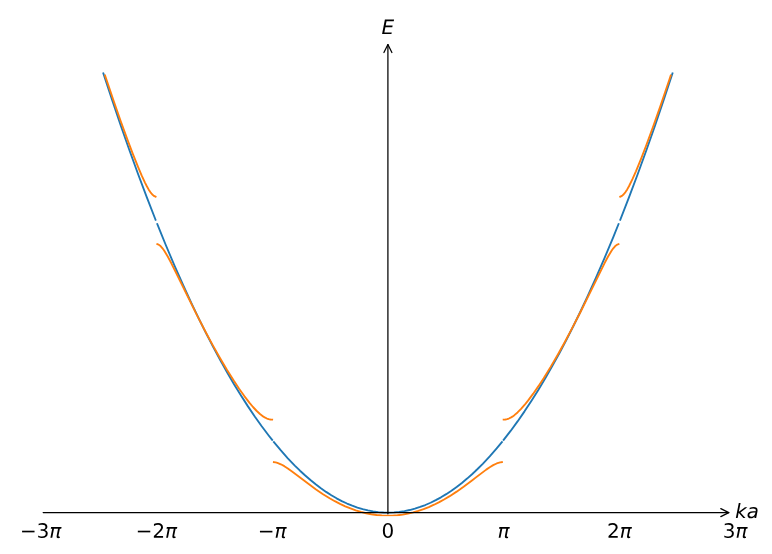
\includegraphics[max width=0.48\linewidth]{ExtendedFreeBands}
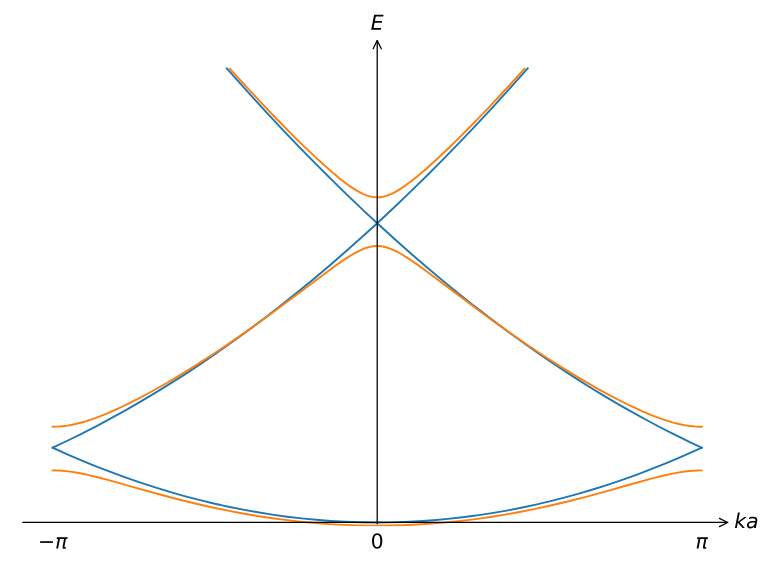
\includegraphics[max width=0.48\linewidth]{ReducedFreeBands}
\caption{Bandas en el esquema de zona extendida (izquierda) y de zona reducida (derecha) para un modelo de electrones totalmente libres y en un potencial periódico débil. Tomados de la referencia \cite{SolidStateCourse}}
\label{fig:bandasFree}
\end{center}
\end{figure}
\section{Modelo de tight-binding}

A continuación vamos a llegar al resultado de interés. En la sección anterior considerábamos un potencial débil. En esta sección vamos a considerar los electrones fuertemente ligados a un núcleo. Para desarrollar más adelante el modelo de Hubbard unidimensional nos interesará desarrollar el modelo de cadena lineal, vamos a seguir tanto el Simons \cite{simon2013oxford} como los apuntes de la asignatura \cite{apuntes}.

Vamos a estudiar el modelo de electrones en una cadena en la que consideramos condiciones de contorno periódicas. Esta construcción se va a basar en la superposición de funciones de onda localizadas en las posiciones de cada núcleo de la red.

Vamos a recurrir entonces tanto al método variacional como a la construcción con combinación lineal de orbitales atómicos (LCAO). Se considera entonces una función de onda variacional de la forma $|\psi\rangle = \sum_n \phi_n |n\rangle$. Vamos a considerar que las funciones atómicas son ortogonales $\langle n | m \rangle = \delta_{n,m}$. Las funciones $|n\rangle$ son las funciones de onda en la celda unidad n-ésima. Podemos encontrar a partir de la ecuación de Schrödinger una ecuación efectiva para los valores de $\phi_n$.

$$
H|\psi\rangle = E|\psi\rangle
$$

Usamos que $1 = \sum_m |m\rangle\langle m|$ y:

$$
H|\psi\rangle = \sum_n H\phi_n|n\rangle = \sum_n \sum_m H \phi_n |m\rangle\langle m|n\rangle = \sum_m H \phi_m |m\rangle = \sum_n E \phi_{n'} |'n\rangle
$$

Aplicando ahora $|n\rangle$ a ambos lados, obtenemos nuestra ecuación de Schrödinger eficaz:

\begin{equation}
\sum_m H_{nm} \phi_m = E\phi_n
\label{eq:effectiveTB}
\end{equation}

Donde $H_{nm} = \langle n | H | m \rangle$ son los elementos de matriz del hamiltoniano. Nuestra función de onda proviene de un principio variacional y podemos mejorar nuestra aproximación considerando varios orbitales en cada posición $|n, \alpha\rangle$ con $\alpha$ yendo desde $1$ hasta el orbital más alto que tengamos. Sin embargo, al añadir muchos orbitales, tenemos que dejar de considerar ortogonalidad, con lo que la ecuación efectiva de Schrödinger se vuelve algo más complicada.

Nuestra ecuación de Schrödinger se podrá escribir entonces como $H_0|m\rangle + V|m\rangle = E|m\rangle$ donde $H_0$ es el hamiltoniano "on-site" del electrón y nos da una energía $\varepsilon_0$ en cada sitio, entonces, los elementos de matriz son de la forma:

\begin{equation}
H_{nm} = \varepsilon_0 \delta_{nm} + \sum_{j \neq m} \langle n | V_j | m \rangle
\label{eq:hamElem}
\end{equation}

Donde tendremos que $V_j$ es el potencial generado por el núcleo j-ésimo y su valor esperado va a dar lugar a un término "hopping" de probabilidad de salto del electrón de un núcleo a otro que será $-t$. El teorema de Bloch nos ayudará cuando resolvamos las bandas de energía puesto que nos bastará con resolver la ecuación efectiva en una celda unidad.

\subsection{Orbitales atómicos sin ortogonalidad}

Vamos a resolver un ejemplo más general en el que tenemos perdida de ortogonalidad. Vamos a considerar entonces que $\langle n | n \rangle = 1$ y $\langle n | m \rangle = S_{nm}$. La ecuación (\ref{eq:effectiveTB}) va a quedar entonces de la siguiente manera:

$$
H|\psi\rangle = \sum_n H\phi_n|n\rangle = \sum_n E \phi_n |n\rangle
$$

Ahora aplicando $|m\rangle$ a ambos lados encontramos la ecuación secular para encontrar la energía, que es un problema de autovalores extendido:

\begin{equation}
\sum_m \phi_m (H_{nm} - ES_{nm}) = 0
\end{equation}

\subsection{Cadena monatómica con dos orbitales}

Esta sección y la de segunda cuantización vienen explicadas en un vídeo de Maurits Haverkort en el que se realiza el desarrollo. Aunque el desarrollo lo he realizado personalmente, el vídeo creo que resulta bastante explicativo. \cite{videoTB}

Continuaremos resolviendo un ejemplo concreto en el que vamos a considerar los orbitales ortogonales y cada celda presenta dos orbitales, tenemos los términos de hopping $t_{AA}$, $t_{BB}$ y $t_{AB}$, además consideraremos que esta interacción es únicamente a primeros vecinos.

Para resolver este tipo de problemas en tight-binding consideramos una función de la forma $\phi_n = \frac{e^{-ikna}}{\sqrt{N}}$, en este caso vamos a suponer que cada una de estas funciones lleva además asociada una constante A o B a cada orbital, tendremos entonces que la ecuación a resolver para las energías es la siguiente:

$$
\left. \begin{array}{c}
A (\varepsilon_A + 2t_{AA}cos(ka)) + 2Bt_{AB}cos(ka) = AE \\
B (\varepsilon_B + 2t_{BB}cos(ka)) + 2At_{AB}cos(ka) = BE
\end{array} \right\}
$$

Nuestras funciones de onda on-site van a ser ahora de la forma siguiente:

$$
|\psi\rangle = \sum_n\frac{e^{-ikna}}{\sqrt{N}}\left(A|n, \alpha\rangle + B|n, \beta\rangle\right) 
$$

Donde $|n, \alpha\rangle$ representa el orbital $\alpha$ en el sitio $n$ y viceversa con el $\beta$. Podremos ver que el sistema de ecuaciones anterior representa un sistema de ecuaciones en A y B que podemos expresar como un problema de autovalores.

$$
\left( \begin{array}{cc}
\varepsilon_A + 2t_{AA}cos(ka) - E & 2t_{AB}cos(ka) \\
2t_{AB}cos(ka) & \varepsilon_B + 2t_{BB}cos(ka) - E
\end{array} \right)\left(\begin{array}{c}
A \\
B
\end{array}\right) = \left(\begin{array}{c}
0 \\
0
\end{array}\right)
$$

Vamos a exigir que este sistema tenga soluciones más allá de la trivial, es decir, vamos a exigir que el valor $E$ sea un autovalor de este sistema..

La ecuación característica que nos va a definir las bandas de energía de este sistema será entonces:

$$
\left(\varepsilon_A + 2t_{AA}cos(ka) - E\right)\left(\varepsilon_B + 2t_{BB}cos(ka)-E\right)-4t_{AB}^2cos^2(ka) = 0
$$

Podemos desarrollar estas ecuaciones para encontrar una expresión de las bandas de energía en función de $k$. El desarrollo no es muy interesante, se lo podemos dar a un programa de cálculo simbólico. Vamos a llamar unas cuantas variables nuevas: $\varepsilon_0 = \varepsilon_A + \varepsilon_B + 2(t_{AA} + t_{BB})cos(ka)$, $\Delta = \varepsilon_A - \varepsilon_B + 2(t_{AA} - t_{BB})cos(ka)$ y $t=2t_{AB}cos(ka)$.

Las bandas de energía tienen la siguiente ecuación:

\begin{equation}
E = \frac{1}{2}\left(\varepsilon_0 \pm \sqrt{4t^2 + \Delta^2}\right)
\label{eq:dosOrbs}
\end{equation}

La forma que tienen estas bandas se puede ver en la figura (\ref{fig:bandasDiorb}).

\begin{figure}[h!]
\begin{center}
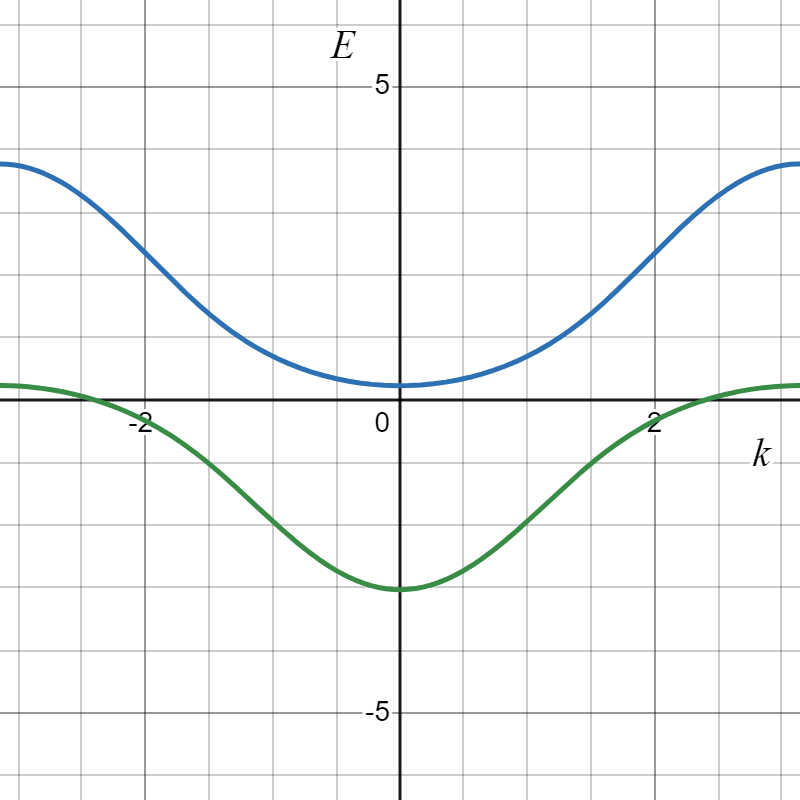
\includegraphics[max width=0.5\linewidth]{Cadena diorbital}
\caption{Bandas que aparecen al resolver una cadena con dos orbitales. Hay que tener en cuenta que cada banda es debido a uno de los dos orbitales considerados. Consideramos las energías on-site diferentes y unos hoppings variados para cada valor.}
\label{fig:bandasDiorb}
\end{center}
\end{figure}

El término de hopping $t_{AB}$ es importante, pues si lo anulamos tendremos dos bandas idénticas, luego, en gran medida, las propiedades de este material vienen marcadas por el hopping cruzado, que le da una forma más interesante a las bandas.

\subsection{Tight-binding en segunda cuantización}

Finalmente, llegamos al resultado más importante de cara a desarrollar el TFG a futuro. Para esta sección nos basaremos en \cite{LuisAVQ} para escribir segunda cuantización. De este documento, podemos recordar que un operador se escribe en su forma de segunda cuantización usando los operadores creación y destrucción de la siguiente manera:

\begin{equation}
H = \sum_{i, j} H_{ij} a_i^{\dagger} a_j
\end{equation}

Recordemos que hay que prestar especial atención en respetar la ordenación normal de estos operadores puesto que podríamos tener problemas con renormalizaciones más adelante.

Si rescatamos ahora la expresión para los elementos de matriz del hamiltoniano en un modelo de tight-binding con funciones de onda atómicas ortogonales (\ref{eq:hamElem}) podemos ver directamente los elementos de matriz, luego, la construcción en segunda cuantización de un hamiltoniano de tight-binding con interacción $-t$ a primeros vecinos y un único orbital se hace de forma muy sencilla. Ahora bien, el teorema de Bloch nos permite resolver el hamiltoniano en una celda unidad puesto en las distintas posiciones la función de onda es periódica, entonces en una celda unidad tenemos que:

\begin{equation}
H = \left(\varepsilon_0 - 2tcos(ka)\right)a_k^{\dagger} a_k
\end{equation}

Y estos operadores nos crean (o destruyen) partículas en el único estado existente posible en el sitio $n$ con vector de onda $k$. Uno puede encontrar las funciones de onda a partir del estado de vacío simplemente encontrando los valores de energía de este hamiltoniano. En este caso, diagonalizar el hamiltoniano nos llevaría a una única banda:

\begin{equation}
E = \varepsilon_0 - 2tcos(ka)
\end{equation}

Y nuestra función de onda sería la siguiente:

\begin{equation}
|\psi\rangle = \sum_n \frac{e^{-ikna}}{\sqrt{N}}a_n^{\dagger}|0\rangle
\end{equation}

Por comparación, la operación $a_k^{\dagger}|0\rangle$ debería de darnos el orbital atómico del sitio $n$, con lo que construimos una función de onda periódica, cumpliendo Bloch. Físicamente, estaríamos creando un único electrón en cada posición de la celda, aunque podríamos crear dos electrones sencillamente considerando el spin, si lo consideramos simplemente hay que añadir otro sumatorio:

\begin{equation}
|\psi\rangle = \sum_{n, \sigma=\uparrow, \downarrow} \frac{e^{-ikna}}{\sqrt{N}}a_{n, \sigma}^{\dagger}|0\rangle
\end{equation}

Así, para cada posición, crearíamos dos electrones con espines opuestos.

\subsection{Cadena monoatómica con dos orbitales en segunda cuantización}

Finalmente, vamos a un caso en el que podemos construir unos autoestados algo más complicados del hamiltoniano. Si recordamos una de las secciones anteriores, resolvimos la energía para una cadena con dos orbitales por átomo (\ref{eq:dosOrbs}).

Por simplicidad vamos a evitar considerar el spin para este ejemplo. El hamiltoniano en segunda cuantización para este sistema se construiría de la siguiente manera:

$$
H = \left(a^{\dagger}_{k \alpha}, a^{\dagger}_{k \beta}\right)\left(\begin{array}{cc}
\frac{\varepsilon_0 + \Delta}{2} & t \\
t & \frac{\varepsilon_0 - \Delta}{2}
\end{array}\right)\left(\begin{array}{c}
a_{k \alpha} \\
a_{k \beta}
\end{array}\right)
$$

Y obtendríamos valores de $A$ y $B$ que nos permiten obtener los autoestados, siendo entonces que las autofunciones de este hamiltoniano sin normalizar serían:

$$
\begin{array}{c}
|\psi_0\rangle = A\left(\frac{\Delta + \sqrt{4t^2 + \Delta^2}}{2} a^{\dagger}_{k\alpha} - ta^{\dagger}_{k\beta}\right)|0\rangle \\
|\psi_1\rangle = A\left(\frac{\Delta + \sqrt{4t^2 + \Delta^2}}{2} a^{\dagger}_{k\beta} + ta^{\dagger}_{k\alpha}\right)|0\rangle
\end{array}
$$

Donde $A$ ahora es una constante de normalización de estos autoestados. En cualquier caso, considerar aquí el spin no sería complicado, puesto que en cada orbital de la posición $n$ podemos crear dos electrones de spines opuestos podremos tener un total de 4 spines, para considerar el spin, tan sólo añadimos la suma de spines al inicio de estas autofunciones.

Es curioso ver que estas dos autofunciones se relacionan por el término $t_{AB}$ pues en cada una de ellas aparecen electrones en otros orbitales. Si no existiese un término de hopping cruzado, tendríamos que cada autofunción sólo presenta probabilidad de electrones en uno de los dos orbitales.

\section{Conclusiones}

Finalmente, alcanzamos el resultado del hamiltoniano de tight-binding en segunda cuantización, haciendo un breve repaso de los modelos más importantes de electrones en sólidos.

Con este hamiltoniano desarrollado podemos avanzar a describir el hamiltoniano de Hubbard y llegar al modelo que queremos desarrollar.

\printbibliography
\end{document}